% 一维波动方程的数值解
% 波动方程|边界条件|有限差分

\pentry{一维波动方程\upref{WEq1D}, Matlab 的判断与循环\upref{MIfFor}}

\footnote{本文参考了 \href{http://hplgit.github.io/num-methods-for-PDEs/doc/pub/wave/sphinx/._main_wave001.html\#discretizing-the-domain}{BCB}}已知一维的波动方程为(\autoref{WEq1D_eq3}\upref{WEq1D})

\begin{equation}
\pdv[2]{y}{x} - \frac{1}{c^2}\pdv[2]{y}{t} = 0
\end{equation}

其中 $y(x, t)$ 是坐标和时间的函数. 这里介绍一个简单的\textbf{有限差分(finite difference)}法, 即把空间 $x$ 和时间 $t$ 划分成等距离的网格 $x_1, \dots, x_{Nx}$ 和 $t_1, \dots, t_{Nt}$, 步长分别为 $\Delta x$ 和 $\Delta t$. 我们将每个格点处的函数值记为 $y_{i,n} = y(x_i, t_n)$

有了网格以后, 我们可以用有限差分表示二阶导数(\autoref{DerDif_eq5}\upref{DerDif})得
\begin{equation}
\frac{y_{i-1,n} - 2y_{i,n} + y_{i+1,n}}{\Delta x^2} - \frac{1}{c^2} \frac{y_{i, n-1} - 2y_{i, n} + y_{i, n+1}}{\Delta t^2} = 0
\end{equation}
整理得
\begin{equation}
y_{i, n+1} = 2y_{i, n} - y_{i, n-1} + C^2(y_{i-1,n} - 2y_{i,n} + y_{i+1,n})
\end{equation}
其中
\begin{equation}
C = c \frac{\Delta t}{\Delta x}
\end{equation}
是一个无量纲得常数. 也就是说, 当我们已知 $t_n$ 和 $t_{n-1}$ 时刻的波函数, 就可以得到 $t_{n+1}$ 时刻的波函数.

\subsection{边界条件}
如果令网格边界处 $y = 0$ (Dirichlet 边界条件) 则会发生全反射且有半波损失. 若边界处使用 $\pdv*{y}{x} = 0$(Neumann 边界条件) 同样会发生全反射但没有半波损失.

另外有一种很有用的边界条件叫 open boundary condition 或者 radiation boundary condition\footnote{\href{http://hplgit.github.io/num-methods-for-PDEs/doc/pub/wave/sphinx/._main_wave003.html\#problem-11-implement-open-boundary-conditions}{查看原文}}, 可以使波动完全不发生反射
\begin{equation}
\pdv{y}{t} + c\pdv{y}{x} = 0
\end{equation}
要验证该条件, 将任何速度为 $c$ 的平面波带入发现都可以满足.

\subsection{Matlab 程序}
程序如下, 运行结果(动画)见 \href{http://wuli.wiki/apps/wavBC.html}{wuli.wiki/apps/wavBC.html}. 截图见\autoref{W1dNum_fig1}.
\Code{wave1D}

\begin{figure}[ht]
\centering
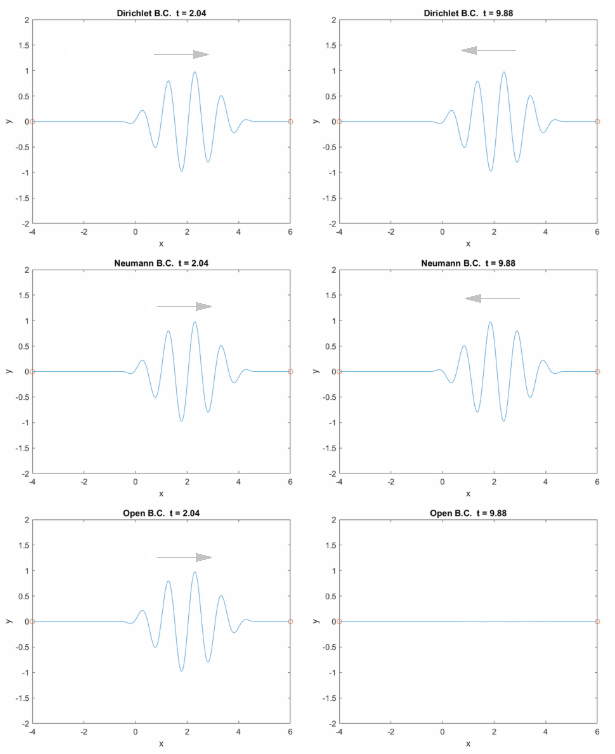
\includegraphics[width=16cm]{./figures/W1dNum1.png}
\caption{运行结果截图, Dirichlet 边界反射后发生相位反转(半波损失), Neumann 边界条件反射后无半波损失, Open 边界条件无反射} \label{W1dNum_fig1}
\end{figure}
